
\documentclass[conference,compsoc]{IEEEtran}


\ifCLASSOPTIONcompsoc
 
  \usepackage[nocompress]{cite}
\else
  % normal IEEE
  \usepackage{cite}
\fi




% *** GRAPHICS RELATED PACKAGES ***
%
\ifCLASSINFOpdf
   \usepackage[pdftex]{graphicx}

\else

\fi



% correct bad hyphenation here
\hyphenation{op-tical net-works semi-conduc-tor}


\begin{document}
%
% paper title
% Titles are generally capitalized except for words such as a, an, and, as,
% at, but, by, for, in, nor, of, on, or, the, to and up, which are usually
% not capitalized unless they are the first or last word of the title.
% Linebreaks \\ can be used within to get better formatting as desired.
% Do not put math or special symbols in the title.
\title{Homework 3  \\ Information Extractor}


% author names and affiliations
% use a multiple column layout for up to three different
% affiliations
\author{\IEEEauthorblockN{Marco Treglia}
\IEEEauthorblockA{ University of Sapienza \\
Master in Artificial Inteligents and Robotics\\
Natural Leanguage Processing }
}


%\IEEEspecialpapernotice{(Invited Paper)}




% make the title area
\maketitle

% As a general rule, do not put math, special symbols or citations
% in the abstract
\begin{abstract}
In this homework, we have to excerpt information from a large set of Wikipedia's corpus. Precisely we have to extract at list twenty triple with the form $t=<a_{i}, r , a_{j}>$ which $a_{i} $ and $a_{j}$ arguments are the entity or concept and $r $ is the relation pattern. We have to submit five relation wich in my case are shape, size, how to use, smell and sound.  Then generate pairs of question-answer for each triple founded corresponding at the respective relation.
\end{abstract}
\IEEEpeerreviewmaketitle

\section{Introduction}
I first start building the DEFIE [1] approach, but at the end, I used differents approaches, respectively for each relation,  on top of the dependency graph. Let's start from the beginning. 

\section{Manage the Data}
For manage, the large dataset close to 19 GBytes compressed. This dataset comprising sixty hundred and sixty-six folder and each folder contains about six thousand and nine hundred XML file representing respectively Wikipedia's article.
For easy oversee this huge dataset I first created the 'DataManager' class [Figure 1]. This first creates an index, then specifying the number of folder and file read the compressed gzip files and then convert it into a more manageable entity named \textbf{Record}. The latter class, in fact, have just two variables inside:
\textit{sentences} are all the phrase of the article, and \textit{sm sentences} are all the babelfy's annotation for each phrase. We can now get into the game. 
\begin{figure}[h]
\centering
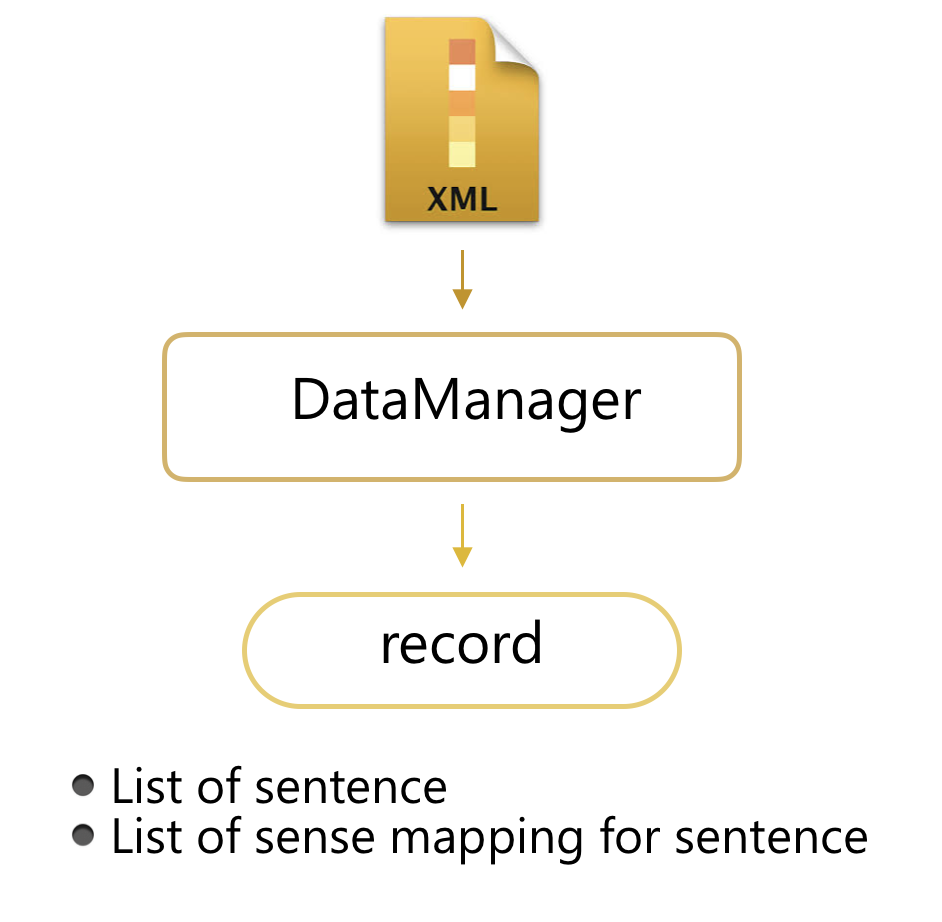
\includegraphics[scale=0.27]{datamanager2}
\caption{ Scheme showing the extraction of data from 'babelfied-wikipediaXML' }
\end{figure}

\section{Dependency extraction}
Having out textual definition \textit{d} we can proceed to the syntactic and semantic analysis.  Looking for the best solution, I came up with some different possibility (Stanford CoreNLP, nltk, spaCy). After some investigations, i chose the open-source library featuring state-of-the-art speed and accuracy spaCy [2].\\
I designed the \textbf{DependencyManager} class, wich takes as input a Record instance and convert each sentence into spacy.tokens.doc.Doc. This provides a nice syntactic analysis but an unprecise semantic parsing. 
For improve it, I merged the words in the spacy tree accordingly to the babelfy annotation. Unfortunately, this framework not provide a graph representation neither then the possibility to get distance or path between the word

 
\section{Dependency graph}
Hence for improve the maneuverability of moving between words in the dependency spacy's tree, I converted it into a graph, using the networkx [3] framework. Accordingly I created the \textbf{GraphManager} class. This class takes as input a DependencyManager instance, wich contains the disambiguated sentence, and create the graph representation. Furthermore, each word is mapped to the class \textbf{Node}, that will be the apt node of the graph. 

\begin{figure}[h]
\centering
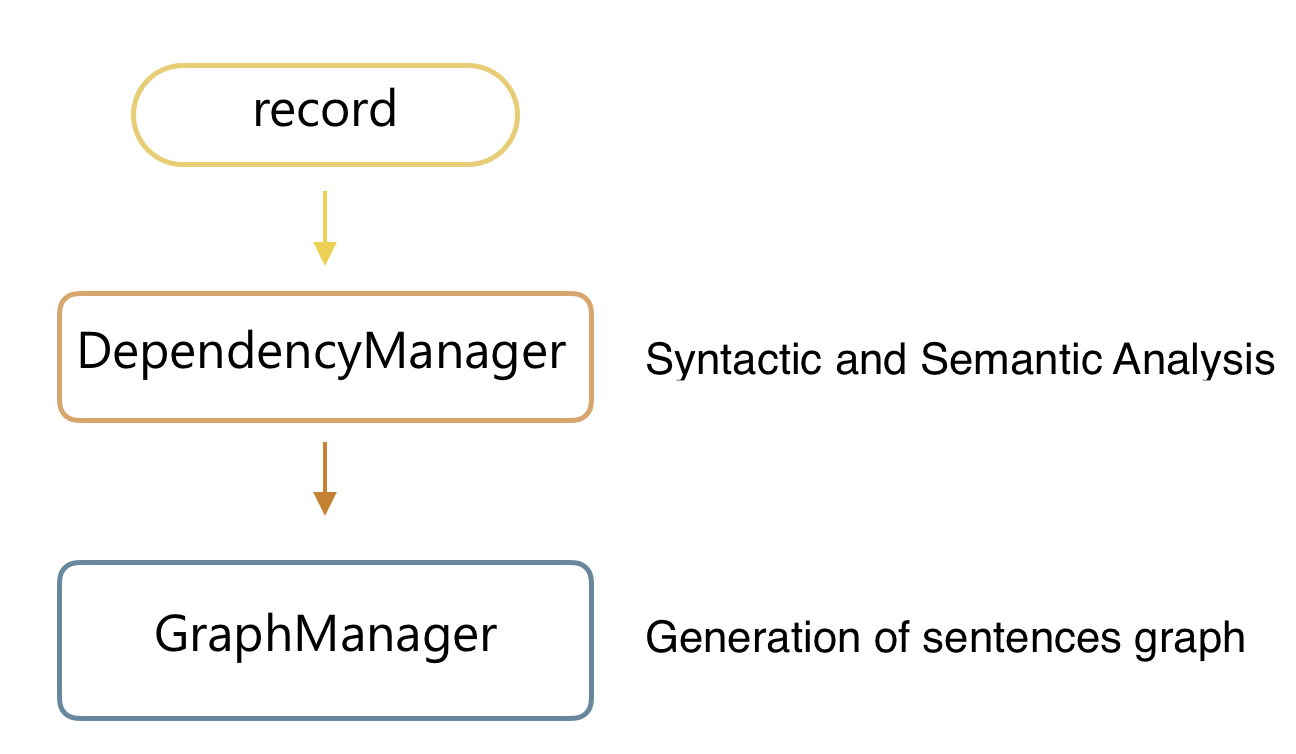
\includegraphics[scale=0.30]{graphmanager2}
\caption{ Scheme showing the generation of the graph }
\end{figure}

\begin{figure}[h]
\centering
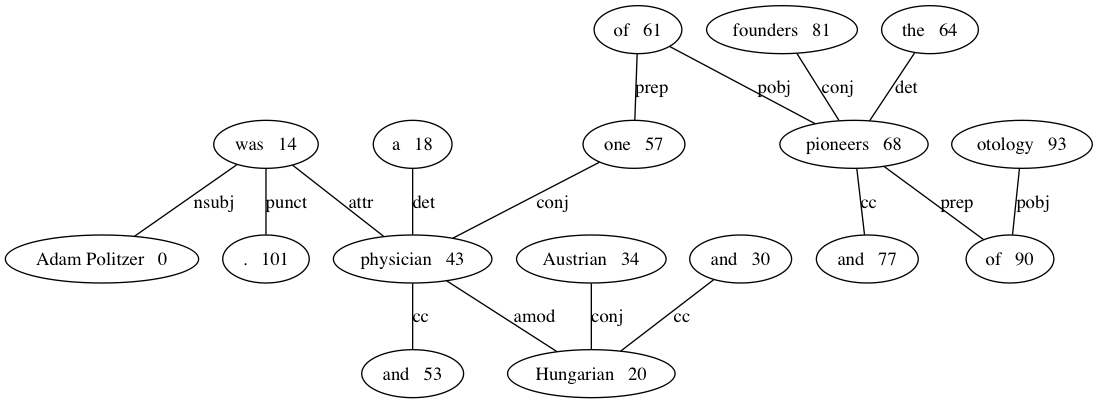
\includegraphics[scale=0.23]{graph}
\caption{ Example graph sentence with semantic tag as edge }
\end{figure}



\section{Triples Extractor}
This is the core of the project, and here comes the tricky thing of getting the right way for extract the information for the respectively relation assigned. The class \textbf{TriplesManager} do all this extraction task, taking as input the graph of the relation and the source text of the latter, then extract,  manage and save each triple founded. For convenience, I used the class \textbf{Triple} for holding the discovered relation.
Here the explanation for each relation.


\begin{figure}[h]
\centering
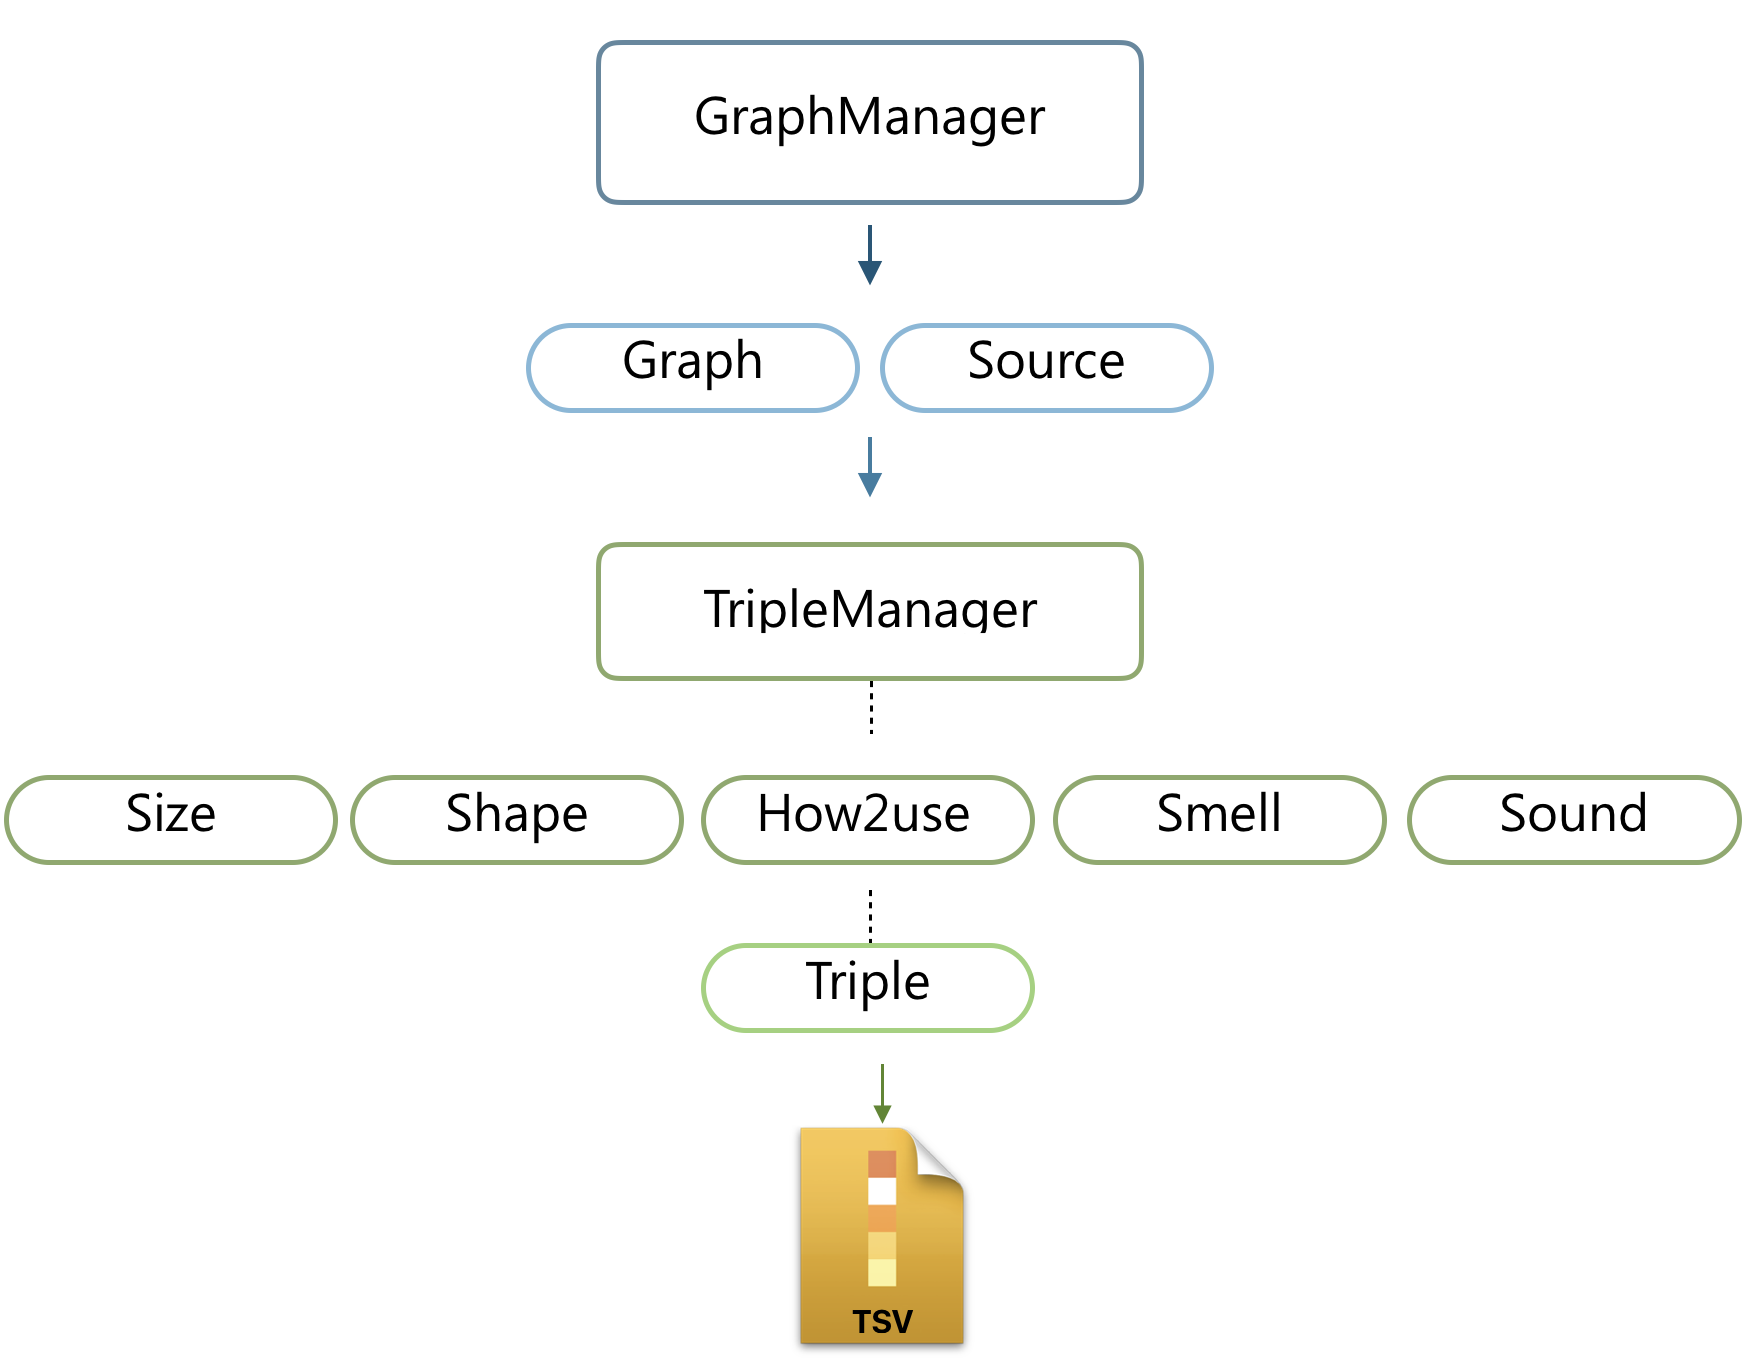
\includegraphics[scale=0.28]{triplemanager}
\caption{ Scheme showing triple's extracion}
\end{figure}



\subsection{Size}
For the extraction of the triples for size relation I first looking in the sentence for all the noun singular and plural using the simpler Google Universal POS (part of speech) tag. Then check if in the sentence there are any adjective that matches with the pattern I used for express the size of something or taking the similarity measure using word2vec vector dimension from this adjective and the word shape.
If the adjective satisfy the pattern or the similarity measure over a thresholder , i take the path between the noun and the adjective and takes only those that are lenght two or maximum three (taking one more word for better express the meanig of the relation with size).

\subsection{Shape}
For the extraction of the triples for shape relation, I used a similar approach for the size relation. Using the same POS noun tag as the first node to check, then verify the existence of an adjective second node which satisfies the similarity over a threshold with shape word or match with some pattern shape adjective. If the requirements are fulfilled, then takes the path between this two node with maximum length as two. \\


\subsection{How to use}
For the extraction of the triples for how to use relation, i used a different approach respect the previous relation. In fact with this, instead searching on the corpus the relation of the noun and a possible verb associate it, I realized that the frequency wich a possible noun (not pronoun) is associated with a verb of the pattern I created is much more likely to be correct respect all the feasible verb that could be found in corpus of reference. So at the beginning, i look for the noun using POS tag, then I measure the similarity between some category pattern I chose and this noun. If is greater than a threshold, I continue with comparing it with some verb pattern selected by me, and again if the similarity exceeds a certain tuned value I produce the triple with the best verb founded. \\



\subsection{Sound}
For the extraction of the triples for sound relation, i used a similar approach to the previous category. In fact, at the begin, i was searching for the phrase with some pattern and I come out with no triples or few incorrect one after several folders inspected. So I move to find a possible pos tag noun in the phrase, then measure the similarity with the pattern category I built. If exceed a threshold, carry on finding again the best fit with my sound adjective pattern. Finally the triple founded belong to the category I determined and contains the best suitable adjective. \\

\subsection{Smell}
For the extraction of the triples for smell relation I realize that was very similar to the sound one. Then using the same category pre-build pattern for making the first selection between the noun I proceed to find the best adjective to express the smell of that entity. I made another pattern for measure the similarity with a common smell-adjective and selected the best one wich, however, overcome the threshold. \\

\section{Question Answer generation}
Finding the triples the task was almost done. For generating the question answer I create a simple class \textbf{QuestionAnswerManager}. At the beginning, i used the triples.tsv file for generating it, but after the delivery requirement update (adding the babel id in the question-answer pair), I change it for generating the pair admitted directly from a Triple instance. In this way, since the Triple instance carries the Node classes, include also the babel id associated with it. I created three patterns for the generation of the question-answer pairs, randomly chosen and, as specify into the submission, I create the wrong question pair using the pattern of respective category. 


\begin{figure}[h]
\centering
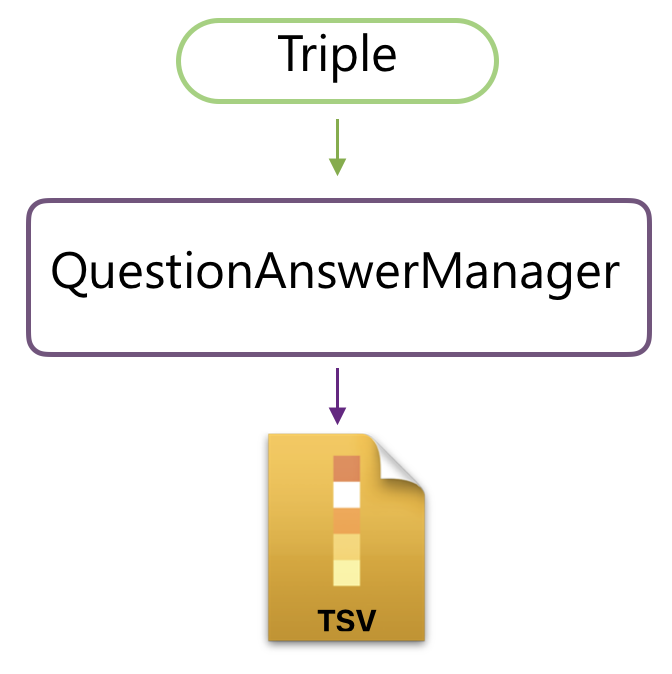
\includegraphics[scale=0.28]{qamanager}
\caption{ Scheme showing question-answer pair generation}
\end{figure}

\section{Statistic}
For easy get the statistic result, I made the \textbf{StatisticAnalysis} class. This reading from the triple founded extract the frequency distribution. \\
\\

\begin{tabular}{rrrrr}
\hline
   shape &   size &   how2use &   smell &   sound \\
\hline
    3888 &  33687 &       473 &      99 &     542 \\
\hline
\end{tabular}


\begin{figure}[h]
\centering
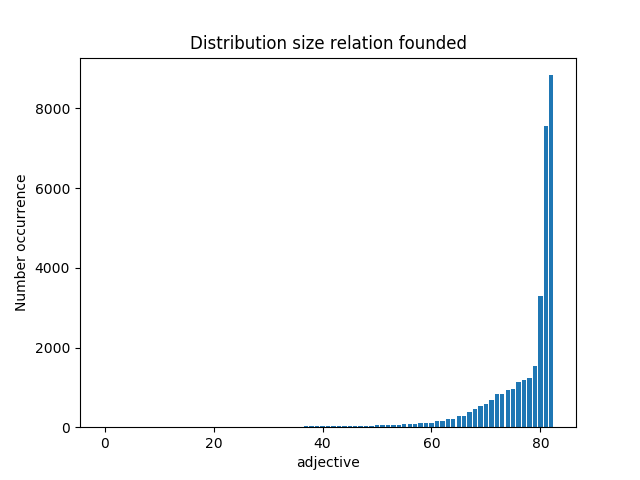
\includegraphics[scale=0.52]{size_plot}
\caption{ Graph showing size adjective distribution}
\end{figure}

Size top ten:
\begin{tabular}{lr}
\hline
 Adjective   &   Frequency \\
\hline
 small       &        8834 \\
 large       &        7553 \\
 short       &        3300 \\
 little      &        1528 \\
 extensive   &        1238 \\
 big         &        1190 \\
 massive     &        1131 \\
 wide        &         953 \\
 huge        &         939 \\
 giant       &         826 \\
 vast        &         825 \\
\hline
\end{tabular}



\begin{figure}[h]
\centering
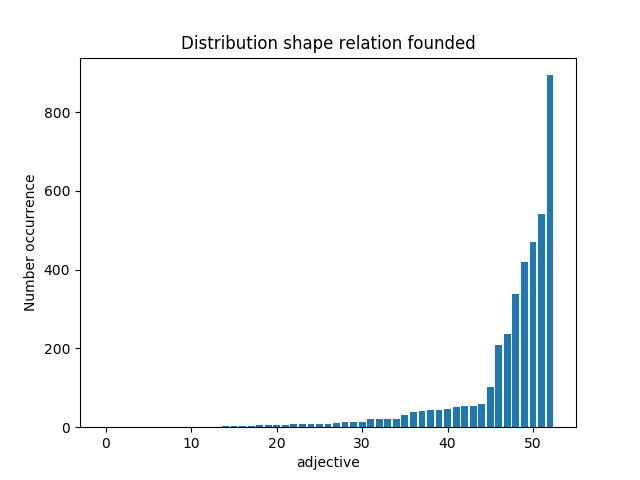
\includegraphics[scale=0.52]{shape_plot}
\caption{ Graph showing shape adjective distribution}
\end{figure}


Shape top ten:
\begin{tabular}{lr}
\hline
 Adjective         &   Frequency \\
\hline
 straight          &         894 \\
 flat              &         542 \\
 closed            &         470 \\
 round             &         419 \\
 solid             &         338 \\
 square            &         236 \\
 rugged            &         210 \\
 curved            &         102 \\
 sweeping          &          58 \\
 three-dimensional &          54 \\
 oval              &          54 \\
\hline
\end{tabular}



\begin{figure}[h]
\centering
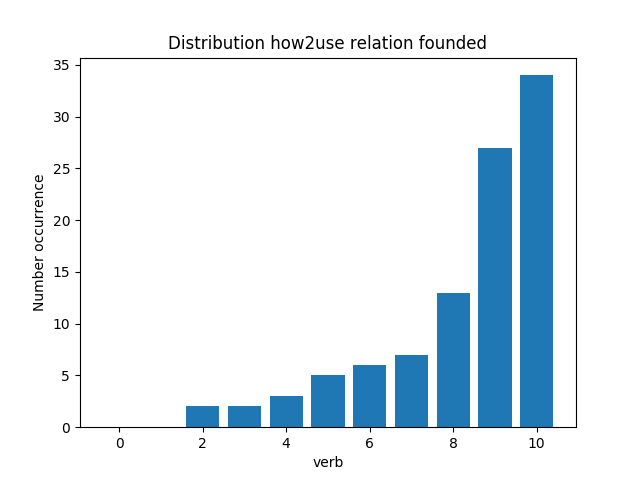
\includegraphics[scale=0.52]{how2use_plot}
\caption{ Graph showing how to use verb distribution}
\end{figure}

How to use  top ten: 
\begin{tabular}{lr}
\hline
 Verb     &   Frequency \\
\hline
 eat      &          34 \\
 cook     &          27 \\
 sing     &          13 \\
 drink    &           7 \\
 read     &           6 \\
 detect   &           5 \\
 shopping &           3 \\
 dance    &           2 \\
 plow     &           2 \\
 activate &           0 \\
 love     &           0 \\
\hline
\end{tabular}

\begin{figure}[h]
\centering
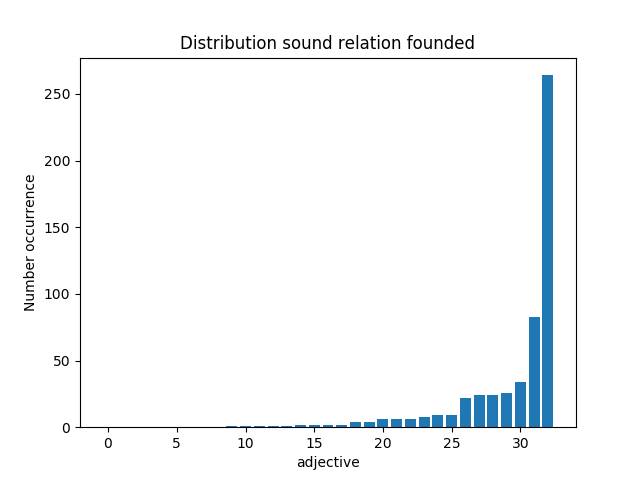
\includegraphics[scale=0.52]{sound_plot}
\caption{ Graph showing sound adjective distribution}
\end{figure}

Sound top ten:
\begin{tabular}{lr}
\hline
 Adjective   &   Frequency \\
\hline
 miaow       &         264 \\
 crunchy     &          83 \\
 strum       &          34 \\
 melodic     &          26 \\
 rhythmic    &          24 \\
 bark        &          24 \\
 bass        &          22 \\
 melodious   &           9 \\
 timbre      &           9 \\
 drone       &           8 \\
 mellifluous &           6 \\
\hline
\end{tabular}



\begin{figure}[h]
\centering
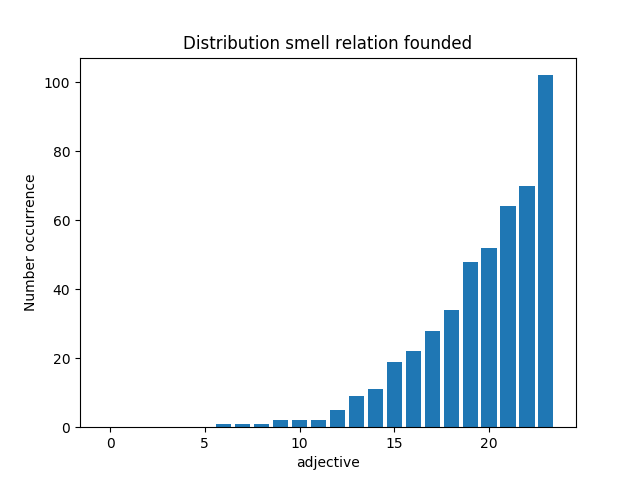
\includegraphics[scale=0.52]{smell_plot}
\caption{ Graph showing smell adjective distribution}
\end{figure}

Smell top ten:
\begin{tabular}{lr}
\hline
 Adjective    &   Frequency \\
\hline
 butterscotch &         102 \\
 musky        &          70 \\
 aromatic     &          64 \\
 fragrant     &          52 \\
 funky        &          48 \\
 perfume      &          34 \\
 honeyed      &          28 \\
 smelly       &          22 \\
 luscious     &          19 \\
 stinky       &          11 \\
 perfumed     &           9 \\
\hline
\end{tabular}


\begin{thebibliography}{1}
\bibitem{IEEEhowto:kopka}
Claudio Delli Bovi, Luca Telesca and Roberto Navigli {Large-Scale Information Extraction from Textual Definitions through Deep Syntactic and Semantic Analysis} .
\bibitem{IEEEhowto:kopka}
https://spacy.io {Industrial-Strength Natural Language Processing} 
\bibitem{IEEEhowto:kopka}
https://networkx.github.io {High-productivity software for complex networks}
\end{thebibliography}




% that's all folks
\end{document}


